\documentclass[openany,10pt]{book}
\usepackage{float}
\usepackage{setspace}
\usepackage{hyperref}
\usepackage{xurl}
\PassOptionsToPackage{hyphens}{url}
\usepackage{hyperref}
\usepackage{amsmath,amsthm,amssymb}
\usepackage[titles]{tocloft}
\usepackage[paperwidth=6in, paperheight=9in, margin=1in]{geometry}
\usepackage{tikz}
\usetikzlibrary{positioning}

\title{Self-Study Guide to Mathematics:\\A Long Road to Baby Rudin}
\date{\today}
\author{Jamie Mellway}
	
\begin{document}
\maketitle

\setlength{\cftbeforechapskip}{3pt}
\tableofcontents

\chapter*{Preface}

This is a strange document.  It started after I was reading some Data Science and Maching Learning books when it became clear that my math was rusty and had holes.  I had a BSc in Physics, so I had some math but nothing in Probability or Statistics.  I should review what I had known and fill in the gaps.  Started looking at MIT OpenCourseWare and other online lectures.  YouTube started recommending me videos by TheMathSorcerer and others that gave recommendations for books.  They leaned on the Proof-Based math textbooks rather than the Computation style course I took as a Physics major.

I started taking down notes on what online lectures I should watch and what textbooks to read.  The notes got rather detailed that they went from hand-written notes to blog posts and then to a \LaTeX document. While I was doing this, I was order tons of math books.  Starting to read them, but mostly studying what to eventually read.  The \LaTeX document grew and started to look like a short book.

This is what you see here.  My plans to self-study mathematics in the future.  Not my notes having read them.  Not being an expert in mathematics or mathematical education.  Plans.

\chapter*{Introduction}


\section*{A Long Road To Baby Rudin}
The hardest course in undergraduate math is taken somewhere in the middle of your studies.  It is Real Analysis and Universities typically use Principles of Mathematical Analysis by Walter Rudin.  The nickname of the book is "Baby Rudin" and his graduate text Real and Complex Analysis is "Papa Rudin".

One could perhaps just jump into reading that book as it starts from first principles and does not have requisites in the normal sense.  However, that would be difficult and if you follow the path here, you will instead be reading over a dozen books just to prepare to tackling it.

\section*{Self-Study vs Augmenting}
The best way to learn mathematics is by doing a degree program at a major University.  That is, with lectures, office hours, graded assignments, and exams.  However, with the availability of University video lectures, course notes, and textbooks, you can get a similar experience.  It is more work doing it yourself, but it is possible.

This book gives suggested books and video courses for mathematics and machine learning.  University video lectures are generally picked over other available videos.  MIT OpenCourseWare video lectures are the main focus of this self-study for mathematics.

Textbooks were selected mainly if they were the book used for a popular video lecture course.  If they are not in print, then the PDF should hopefully be available.

Problem sets are required to learning mathematics.  We will be mainly using textbooks, so they will be filled with problems.  Schaum Outline series of books will also be recommended to add more problems.

I assume there are three main types of people reading this book.  Those that are about to start a degree in Math, Physics, or Engineering looking ahead.  Those part way through a degree looking at current and upcoming courses.  Those who have a related degree already looking to fill in gaps.  That is, people looking for Self-Study to supplement or enhance their formal education.

Another type of reader could be someone approaching Self-Study without any formal higher education at all, but they are in for much more work.  Perhaps the book should have been entitled Supplemental Guide to Mathematics, but we are looking are Core courses rather than supplemental material.

If you are a high school student wanting a head start, my main piece of advice is to work on problem sets everyday.  Get a exercise book on trigonometry, high school algebra, high school calculus, or high school physics and get into the practice of doing exercises everyday.  Beyond that take a look at the Introduction chapter and get one of the books mentioned there.  Getting introduced to proofs early will help out in your lower levels.

If your a student in your lower years, you might be struggling with the concepts or the assignments.  For concepts, it might be helpful to use available online lectures or other textbooks to get a different perspective on the material.  For assignments, you might be looking for more exercises to work on or you might just need to seem some examples with solutions.

\section*{The Curriculum}

A typical University lower level curriculum might look like this.  Taking Calculus 1 and then Calculus 2.  Calculus 2 opening up courses such as Probability, Linear Algebra, and Mathematical Reasoning. Calculus would lead to a course in differential equations.  Probability and Statistics might be one or two courses.  Discrete Math might be available right away or it might require a prerequisite.  Then you're ready to tackle Real Analysis and "Baby Rudin".
\begin{figure}[H]
	\centering
	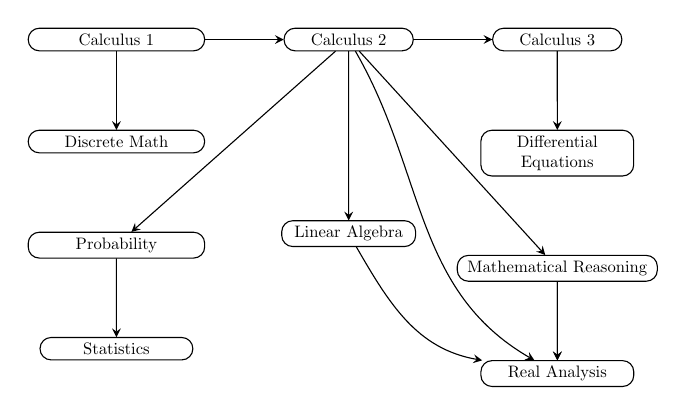
\begin{tikzpicture}[>=stealth,scale=0.6,every node/.style={shape=rectangle,draw,rounded corners,scale=0.6},]
		% create the nodes
		\node (pbc1) [text width=3.5cm, align = center]{Calculus 1};
		%\node (space1) [draw=none,right =of pbc1,align=left] {};
		\node (pbc2) [right =of pbc1,text width=2.5cm, align = center]{Calculus 2};
		
		\node (pbc3) [right =of pbc2,text width=2.5cm, align = center]{Calculus 3};
		\node (space2) [draw=none,below =of pbc2,align=left] {};
		\node (pbla) [below =of space2,text width=2.6cm, align = center]{Linear Algebra};
		\node (dm) [below =of pbc1,text width=3.5cm, align = center]{Discrete Math}; 
		\node (dfe) [below =of pbc3, text width=3cm, align = center]{Differential Equations};
		\node (proofs) [below =of dfe,text width=4cm, align = center]{Mathematical Reasoning};
		\node (ra) [below =of proofs,text width=3cm, align = center]{Real Analysis};
		%\node (ms) [below =of stat,text width=3.7cm, align = center]{Mathematical Statistics\\18.655 Graduate};
		%\node (st) [below =of ra]{Statistical Theory};
		
		
		\node (prob) [below =of dm, text width=3.5cm, align = center]{Probability};
		\node (stat) [below =of prob,text width=3cm, align = center]{Statistics};
		
		% connect the nodes
		\draw[->] (proofs) to (ra);
		\draw[->] (pbc1) to (pbc2);
		\draw[->] (pbc1) to (dm);
		\draw[->] (pbc2) to (pbc3);
		\draw[->] (pbc2) to (pbla);
		\draw[->] (pbc2) to (prob);
		\draw[->] (pbc3) to (dfe);
		\draw[->] (prob) to (stat);
		\draw[->] (pbc2) to (proofs);
		\draw[->] (pbc2) to[out=300,in=150] (ra);
		\draw[->] (pbla) to[out=300,in=170] (ra);
		\draw[->] (proofs) to (ra);
		
		%\node[draw=none,align=left] at (2,1) {Proof-Based};
		
		%\draw [dotted] (-2,.7) -- (8,.7);
		
	\end{tikzpicture}
	\caption{Lower Years Core Curriculum} \label{fig:M1}
\end{figure}

The watershed moment in a math students path is Real Analysis.  A lot of the lower level courses are preparing you for Real Analysis.  Once you have taken Real Analysis, most of the upper level courses will become available to you as have Real Analysis will be a prerequisite.  It is not so much that the material is required, but having got through Real Analysis means that you are ready to handle upper level courses. We will also look at the upper year courses you could take.  

After doing Real Analysis, it is also a good time to start looking at books such as the Princeton Companions or general surveys.  These will be looked at in part VIII. 

\begin{figure}[H]
	\centering
	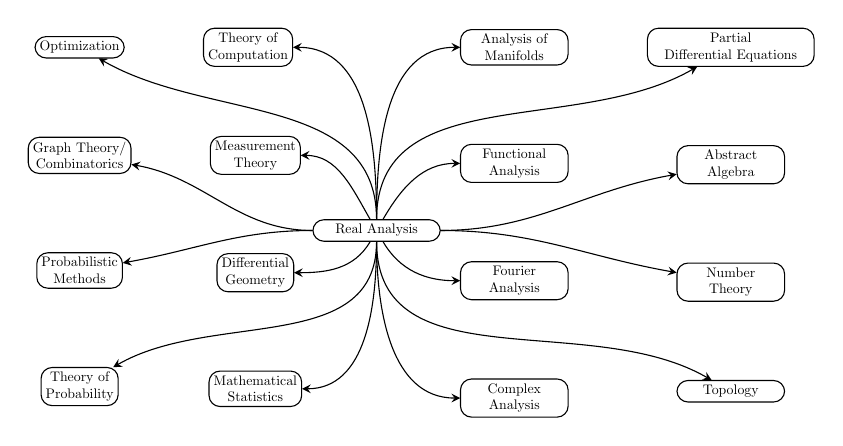
\begin{tikzpicture}[>=stealth,scale=0.5,every node/.style={shape=rectangle,draw,rounded corners,scale=0.5},]
		% create the nodes
		\node (n1) [align=left] {Optimization};
		\node (n2) [right =of n1, align=center] {Theory of\\Computation};
		\node (n3) [below =of n1, align=center] {Graph Theory/\\Combinatorics};
		\node (n4) [right =of n3, align=center] {Measurement\\Theory};
		\node (n5) [below =of n3, align=center] {Probabilistic\\Methods};
		\node (n6) [below =of n4, align=center] {Differential\\Geometry};
		\node (n7) [below =of n5, align=center] {Theory of\\Probability};
		\node (n8) [below =of n6, align=center] {Mathematical\\Statistics};
		
		\node (space1) [right =of n2, draw=none,align=left] {};
		\node (space2) [draw=none,below =of space1,align=left] {};
		\node (space3) [draw=none,below =of space2,align=left] {};
		
		\node (ra) [text width=3cm, below =of space2, align = center]{Real Analysis};
		\node (aam) [right =of space1,text width=2.5cm, align = center]{Analysis of Manifolds};
		\node (functional) [below =of aam,text width=2.5cm, align = center]{Functional Analysis};
		\node (fourier) [below =of functional,text width=2.5cm, align = center]{Fourier Analysis};
		\node (complex) [below =of fourier,text width=2.5cm, align = center]{Complex Analysis};
		
		\node (pde) [right =of aam,text width=4cm, align = center]{Partial\\Differential Equations};
		\node (abstract) [below =of pde,text width=2.5cm, align = center]{Abstract Algebra};
		\node (number) [below =of abstract,text width=2.5cm, align = center]{Number\\Theory};
		\node (topology) [below =of number,text width=2.5cm, align = center]{Topology};
		
		
		% connect the nodes
		\draw[->] (ra) to[out=90,in=330] (n1);
		\draw[->] (ra) to[out=90,in=0] (n2);
		\draw[->] (ra) to[out=180,in=350] (n3);
		\draw[->] (ra) to[out=120,in=0] (n4);
		\draw[->] (ra) to[out=180,in=10] (n5);
		\draw[->] (ra) to[out=240,in=0] (n6);
		\draw[->] (ra) to[out=270,in=30] (n7);
		\draw[->] (ra) to[out=270,in=0] (n8);
		
		
		\draw[->] (ra) to[out=90,in=180] (aam);
		\draw[->] (ra) to[out=60,in=180] (functional);
		\draw[->] (ra) to[out=300,in=180] (fourier);
		\draw[->] (ra) to[out=270,in=180] (complex);
		\draw[->] (ra) to[out=90,in=210] (pde);
		\draw[->] (ra) to[out=0,in=190] (abstract);
		\draw[->] (ra) to[out=0,in=170] (number);
		\draw[->] (ra) to[out=270,in=150] (topology);
		
	\end{tikzpicture}
	\caption{Upper Years Math Core Curriculum} \label{fig:M2}
\end{figure}

\section*{Computation vs Proof-Based}

Those with degrees in Physics and Engineering have taken a lot of math courses, but they probably haven't taken the proof-based versions them.  Their path might be to re-take Calculus or Linear Algebra with different textbooks, study Real Analysis, and then start filling in their gaps with upper level mathematics.\newline

There are two or more streams that you can go down.  You will be given an option to take either the Computation versions of the course or a Proof-Based version of the course.  They will be anti-requisites to each other so you can only take one version of the course for credit.  Those in Applied programs such as Physics or Engineering will typically the computation stream and Mathematics majors will take the Proof-Based version.

\begin{figure}[H]
	\centering
	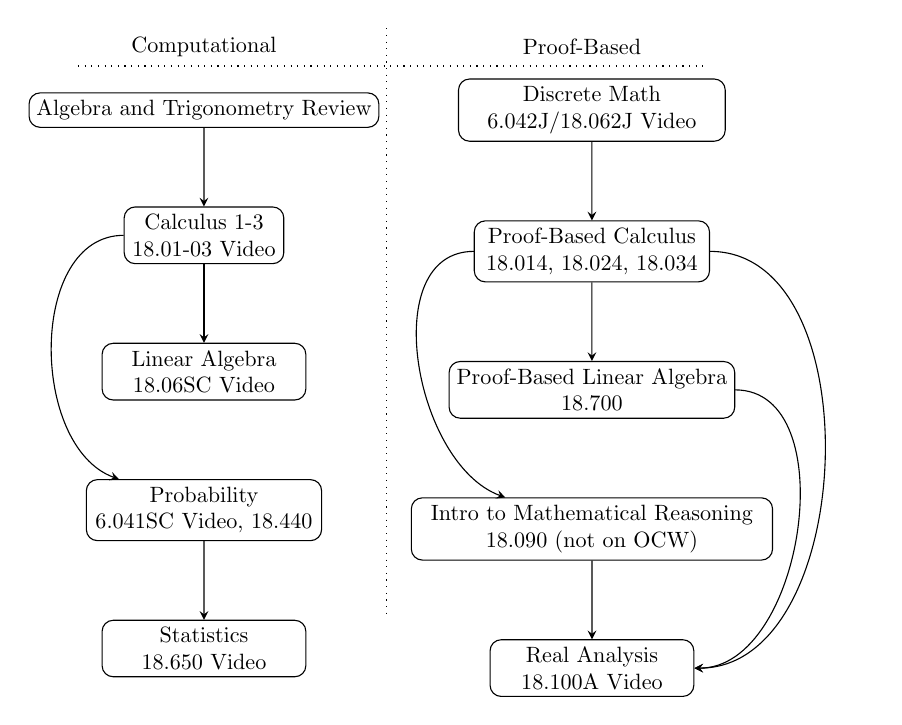
\begin{tikzpicture}[>=stealth,scale=0.8,every node/.style={shape=rectangle,draw,rounded corners,scale=0.8},]
		% create the nodes
		\node (at) {Algebra and Trigonometry Review};
		\node (dm) [right =of at,text width=4cm, align = center]{Discrete Math\\6.042J/18.062J Video}; 
		\node (c) [below =of at,text width=2.3cm, align = center]{Calculus 1-3\\18.01-03 Video};
		\node (pbc) [below =of dm,text width=3.5cm, align = center]{Proof-Based Calculus\\18.014, 18.024, 18.034};
		\node (la) [below =of c,text width=3cm, align = center]{Linear Algebra\\18.06SC Video};
		\node (pbla) [below =of pbc,text width=4.3cm, align = center]{Proof-Based Linear Algebra\\18.700};
		\node (proofs) [below =of pbla,text width=5.5cm, align = center]{Intro to Mathematical Reasoning\\18.090 (not on OCW)};
		\node (ra) [below =of proofs,text width=3cm, align = center]{Real Analysis\\18.100A Video};
		\node (prob) [below =of la,text width=3.5cm, align = center]{Probability\\6.041SC Video, 18.440};
		\node (stat) [below =of prob,text width=3cm, align = center]{Statistics\\18.650 Video};
		%\node (ms) [below =of stat,text width=3.7cm, align = center]{Mathematical Statistics\\18.655 Graduate};
		%\node (st) [below =of ra]{Statistical Theory};
		
		% connect the nodes
		\draw[->] (at) to (c);
		\draw[->] (dm) to (pbc);
		\draw[->] (proofs) to (ra);
		\draw[->] (c) to (la);
		\draw[->] (prob) to (stat);
		\draw[->] (pbc) to (pbla);
		\draw[->] (c) to[out=180,in=160] (prob);
		\draw[->] (pbc) to[out=180,in=160] (proofs);
		\draw[->] (pbc) to[out=0,in=0] (ra);
		\draw[->] (pbla) to[out=0,in=0] (ra);
		%\draw[->] (proofs) to[out=0,in=0] (ra);
		
		\node[draw=none,align=left] at (0,1) {Computational};
		\node[draw=none,align=left] at (6,1) {Proof-Based};

	\draw [dotted] (2.9,1.3) -- (2.9,-8);
	\draw [dotted] (-2,.7) -- (8,.7);
		
	\end{tikzpicture}
	\caption{Separate Core Curriculums} \label{fig:M3}
\end{figure}

The video lectures that are available online are generally Applied Math/computation versions of the course.  Also, the applied or computation courses are generally easier.  In this Self-Study guide we will be looking at both versions.  We will take an Applied-first approach where we look at the applied version of the topic and then later (and optionally) the Pure Proof-Based approach.  If you are looking for just a Applied approach, you can just do the Computation chapters and skip the Proof-Based ones.  If you are doing Pure math, you would want to at least read the applied chapters and study the pure math chapters.

\begin{figure}[H]
\centering
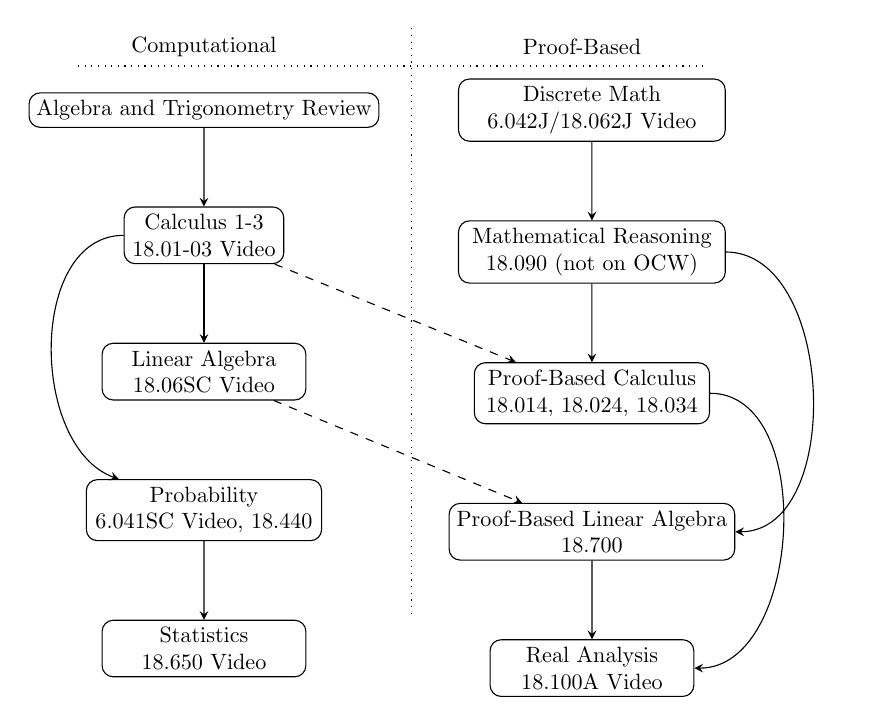
\begin{tikzpicture}[>=stealth,scale=0.8,every node/.style={shape=rectangle,draw,rounded corners,scale=0.8},]
	% create the nodes
	\node (at) {Algebra and Trigonometry Review};
	\node (dm) [right =of at,text width=4cm, align = center]{Discrete Math\\6.042J/18.062J Video}; 
	\node (proofs) [below =of dm,text width=4cm, align = center]{Mathematical Reasoning\\18.090 (not on OCW)};
	\node (c) [below =of at,text width=2.3cm, align = center]{Calculus 1-3\\18.01-03 Video};
	\node (pbc) [below =of proofs,text width=3.5cm, align = center]{Proof-Based Calculus\\18.014, 18.024, 18.034};
	\node (la) [below =of c,text width=3cm, align = center]{Linear Algebra\\18.06SC Video};
	\node (pbla) [below =of pbc,text width=4.3cm, align = center]{Proof-Based Linear Algebra\\18.700};
	\node (ra) [below =of pbla,text width=3cm, align = center]{Real Analysis\\18.100A Video};
	\node (prob) [below =of la,text width=3.5cm, align = center]{Probability\\6.041SC Video, 18.440};
	\node (stat) [below =of prob,text width=3cm, align = center]{Statistics\\18.650 Video};
	%\node (ms) [below =of stat,text width=3.7cm, align = center]{Mathematical Statistics\\18.655 Graduate};
	%\node (st) [below =of ra]{Statistical Theory};
	
	% connect the nodes
	\draw[->] (at) to (c);
	\draw[->] (dm) to (proofs);
	\draw[->] (proofs) to (pbc);
	\draw[->] (c) to (la);
	\draw[->,dashed] (la) to (pbla);
	\draw[->,dashed] (c) to (pbc);
	\draw[->] (c) to[out=180,in=160] (prob);
	\draw[->] (prob) to (stat);
	%\draw[->] (stat) to (st);
	\draw[->] (pbla) to (ra);
	\draw[->] (pbc) to[out=0,in=0] (ra);
	\draw[->] (proofs) to[out=0,in=0] (pbla);
	%\draw[->] (proofs) to[out=0,in=0] (ra);
	%\draw[->] (stat) to (ms);
	%\draw[->] (ra) to (st);
	
	\node[draw=none,align=left] at (0,1) {Computational};
	\node[draw=none,align=left] at (6,1) {Proof-Based};
	
	\draw [dotted] (3.3,1.3) -- (3.3,-8);
	\draw [dotted] (-2,.7) -- (8,.7);
\end{tikzpicture}
\caption{Computational-First, Proofs-First Core Curriculum} \label{fig:M4}
\end{figure}

What I'll do in each chapter is give suggested textbooks and video lecture series for the topic.  I'll go into detail in what the they cover.  

I'll spell out most of the definitions and theorems as appropriate.  This will be super fast and dense reading.  You will not be expected to learn or memorize the definitions and theorems, but it will give you a quick run down on what is covered and could be used as a review afterwards.  This book is a long cheat sheet.


\part{General}

\part{Starting Points}

\chapter{Algebra and Trigonometry Review}

Recommended Book: Algebra and Trigonometry by Sullivan\newline

\noindent \textit{Workbooks}: Schaum Outline of Precalculus, Schaum Outline of Trigonometry\newline

\noindent In University, you are expected to already know high school and college math.  It is everywhere and it will not be reviewed in detail and so you might need to spend some time getting this down.  It is not enough to just know it, but it should be lightning fast.  Many University Physics problems have a trigonometry component and so if you are slow at trig and need to use your cheat sheet, you will be slow at Physics problems even if you have the Physics bits down cold.

There are levels of difficulty in Algebra books each with their own textbooks.\newline
1. Pre-Algebra\newline
2. Elementary Algebra\newline
3. Intermediate Algebra\newline
4. College Algebra\newline
5. Pre-Calculus (Algebra and Trigonometry)\newline
6. Higher Algebra\newline
7. Classical Algebra\newline

Pre-Algebra deals with... 

Elementary Algebra covers...

Intermediate Algebra covers...

College Algebra covers...

Pre-Calculus (also called "Algebra and Trigonometry") is likely the level you want to review before starting the University curriculum.

Higher Algebra is something which is not really found in Western countries.

Classical Algebra is the name for the first math course I had at Waterloo.  It covers...

Trigonometry is concerned with the measurement of the parts, sides, and angels of a triangle.  plane trigonometry is restricted to triangles lying in a plane.  A plane angle is formed by two rays.  The point is the vertex and the lines are the sides.  When revolving a ray from the initial position to the terminal position, the lines are called the initial side and the terminal side.  The angle is positive if it is rotated counter-clockwise and negative if clockwise.

\chapter{Introduction to Math}

Two books that would be of interest to high school students preparing for University are 'How To Think Like A Mathematician' by Houston and 'How to Study as a Mathematics Major' (that is the UK version, it is also published as 'How to Study for a Mathematics Degree' in the US) by Lara Alcock.  They are a mix of informal advice and introducing discrete math and proofs.  These aren't textbooks and both can be read more like a novel although Housten has a few textbook like chapters.

There is informal advise on reading mathematics, writing mathematics, solving problems, understanding proofs.  Alcock also has advise on attending lectures, interacting with professors, time management, and getting behind.

You will learn about \textbf{sets} which are a well-defined collection of objects.  A \textbf{element} is an object in a set.  $\varnothing$ is the empty set.  If $x$ is an element of $X$ we write $x\in X$ and we say $\in$ as 'in'.  Not in is $x\notin X$. Sets $X$ and $Y$ are \textbf{equal} if they have the same elements which we write as $X=Y$.  Not equal is $X\neq Y$. If a set have finite number of elements it is a \textbf{finite set}.  The number of elements is the \textbf{cardinality} and is denoted $|X|$.  X is a subset of Y if every element in X is also in Y and is written as $X\subseteq Y$.  X is a \textbf{proper subset} of Y if $X\subseteq Y$ and X is not equal to Y and is denoted by $X\subset Y$.  

Can also use set notation $\{x|x$ satifies propery $P\}$.  The $|$ is read as "such that". The \textbf{union} of $X$ and $Y$, written $X\cup Y$, is the set consisting of elements that are in at least one of $X$ or $Y$.  We can define the set as $X\cup Y = \{x|x\in X$ or $x\in Y\}$.  The \textbf{intersection} of $X$ and $Y$, written $X\cap Y$, is the set consisting of elements that are in both $X$ and $Y$.  We can define the set as $X\cap Y = \{x|x\in X$and $x\in Y\}$.

The \textbf{difference} of $X$ and $Y$, written $X\backslash Y$, is the set of elements that are in $X$ but not in $Y$.  If $Y$ is also a subset of $X$, then we often call $X\backslash Y$ the \textbf{complement} of $Y$ in $X$ and denote this by $Y^C$.

You will learn that the set of \textbf{natural numbers} is $\{1,2,3,4,\ldots\}$ is denoted by $\mathbb{N}$.  The set of \textbf{integers} is $\{\ldots,-4,-3,-2,-1,0,1,2,\\3,4,\ldots\}$ is denoted by $\mathbb{Z}$.  The set of \textbf{rational numbers} consisting of all fractional numbers is denoted by $\mathbb{Q}$.  \textbf{Irrational numbers} includes non-repeating decimal numbers such as $\pi$, $\sqrt{2}$, and $e$.  The set of \textbf{real numbers} include both rational and irrational numbers is denoted by $\mathbb{R}$.  The set of \textbf{complex numbers} aren't covered, but they are denoted by $\mathbb{C}$.

The \textbf{product} of $X$ and $Y$, denoted $X\times Y$ is the set of all possible pairs $(x,y)$ where $x\in X$ and $y \in Y$, i.e. $X \times Y = \{(x,y)|x\in X$ and $y\in Y\}$.  

A \textbf{function} or \textbf{map} from X to Y is an association where for every element of $X$ there is a unique element of $Y$.  If $f$ is a function from X to Y, then we write $f:X\rightarrow Y$, and the unique elements in Y associated to x is denoted $f(x)$.  This element is called the \textbf{value of $x$ under $f$} or called a \textbf{value} of $f$.  The set $X$ is called the \textbf{source} (or \textbf{domain}) of $f$ and $Y$ is called the \textbf{target} (or \textbf{codomain}) of $f$.

You will learn about logic.  That a \textbf{statement} is a sentence that is either true or false.  The \textbf{law of excluded middle} prevents an fuzzy or indeterminate statements.  A \textbf{negation}.... Logical And and logical or.  \textbf{Implications}.  \textbf{Inverse}.  \textbf{Necessary and sufficient conditions}.    \textbf{Converse}. \textbf{Contrapositive}. Quantifiers

You will learn about definitions, theorems, lemmas, proofs, conjectures, and axioms.

\noindent \textbf{Definition:} A number $n$ that is \textbf{even} if $\exists k\in\mathbb{Z}$ such that  $n = 2k$. \newline
\noindent \textbf{Definition:} A function $f:\mathbb{R}\rightarrow\mathbb{R}$ is \textbf{increasing} if $\forall x_1, x_2\in\mathbb{R}$ such that $x_1<x_2$, we have $f(x_1)\leq f(x_2)$.\newline
\noindent \textbf{Definition:} A binary operation * on a set S is \textbf{communtative} if $\forall$ elements $s_1$ and $s_2$ in $S$, $s_1*s_2=s_2*s_1$.\newline
\noindent \textbf{Definition:} A set $X\subseteq \mathbb{R}$ is \textbf{open} if $\forall x\in X \exists d>0$ such that $(x-d,x+d) \subseteq X$.\newline
\noindent \textbf{Definition:}(p 52)\newline
\noindent \textbf{Definition:}(p 62)\newline
\noindent \textbf{Definition:}(p 63)\newline
\noindent \textbf{Definition:}(p 66)\newline
\noindent \textbf{Definition:}(p 66)

\noindent \textbf{Theorem:} If $l$,$m$, and $n$ are consecutive integers, then the product $lmn$ is divisible by 6.\newline
\noindent \textbf{Theorem:} If f is an even function, then df/dx is an odd function.\newline
\noindent \textbf{Theorem:} If $ax^2 +bx+c=0$, then $x=\frac{-b+\sqrt{b^2-4ac}}{2a}$.\newline
\noindent \textbf{Theorem:}\newline

Some theorems will be looked including 

You will learn about proofs.  There are five types covered in Houston: direct method, proof by cases, contradiction, induction, and contrapositive method.  \textbf{Proof by induction} is where to show that $P(n)$ is true $\forall n\in \mathbb{N}$, $A(1)$ is true and $A(k)\Rightarrow(k+1)$ is true $\forall k \in \mathbb{N}$.

Functions.  One-to-one or injective.  Onto or surjective.  Inverse function.  Increasing functions.  Even functions. 


\chapter{Discrete Mathematics}

\textit{Books}: Discrete Mathematics with Applications by Epp, Discrete Mathematical Structures by Kolman, Busby, and Ross, MIT OCW 6.042J Textbook (https://ocw.mit.edu/courses/6-042j-mathematics-for-computer-science-spring-2015/pages/readings/)

\noindent \textit{Recommended Course}: MIT OCW 6.042J Mathematics for Computer Science\newline

\noindent A course on discrete mathematics might be called something different at your University such as Classical Algebra,  Mathematics for Computer Science, or Elements of Higher Mathematics.

It will cover such topics as sets, logic, and proofs.  Proofs is a vitally important topic for pure mathematics study, so we'll cover it in detail in the next chapter.


\chapter{Proofs}

\textit{Books}: Mathematical Proofs: A Transition to Advanced Mathematics by Chartrand, Proofs: A Long-Form Mathematics Textbook by Cummings, How to Prove It: A Structured Approach by Velleman

\textit{Videos}: \url{https://www.youtube.com/watch?v=nGEUOLCYbng} (Based on Hammack)

\part{Calculus}

\chapter{Applied Single Variable Calculus}

\textit{Recommended Book}: \newline

\noindent \textit{Course Notes}: Waterloo Math 137

\noindent \textit{Recommended Course}: MIT OCW 18.01SC Single Variable Calculus\newline

\noindent \textit{Alternate Books}: We can use other big books of Calculus by Stewart; Larson and Edwards; or Briggs, Cochran, Gillett, and Schulz.  They might be split up into single and multi-variable volumes.  They might have an Early Transcendental edition and a regular edition.  Early Transcendental just means the section of logarithms appears earlier.  (We'll be using Spivak or Apostol Calculus books in a later chapter.) 

\noindent There is no official textbook for the OpenCourseWare videos, the textbook that MIT used during this period was Introduction to Linear Algebra by Strang.  It is out of print while I am writing this, but it is available as a free PDF.  You might be able to find a used copy.

\chapter{Applied Multivariable Calculus}

\textit{Recommended Book}: \newline

\noindent \textit{Recommended Course}: MIT OCW 18.02SC Multivariable Calculus \newline

\chapter{Vector Analysis}

\textit{Recommended Book}: \newline

\chapter{Differential Equations}

\textit{Recommended Book}: Differential Equations by Zill\newline

\noindent \textit{Recommended Course}: MIT OCW 18.03SC Differential Equations\newline

\part{Linear Algebra}

\chapter{Linear Algebra 1}

\textit{Recommended Book}: Introduction to Linear Algebra by Strang\newline

\noindent \textit{Recommended Course}: MIT OCW 18.06SC Linear Algebra\newline

\noindent \textit{Alternative Courses}: There are 8 lectures by Herb Gross from the 1972 that have been releases through MIT OpenCourseWare.  3brown1blue has around 2 hours in the Linear Algebra series.  Khan Academy has a series on Linear Algebra.  \newline

\noindent \textit{Exams and Problem Sets}: \url{https://web.mit.edu/18.06/www/old.shtml}

\noindent \textit{Prerequisites}: While there is a prerequisite on 18.02 for this course, it is more that they like their students to have gone through Calculus 2 than there being needed knowledge from the course.

\part{Probability and Statistics}

\chapter{Probability}

\textit{Books}: Introduction to Probability by Grinstead and Snell (\url{https://math.dartmouth.edu/~prob/prob/prob.pdf}), Introduction to Probability for Data Science by Stanley Chan, Introduction To Probability by Bertsekas and Tsitsiklis (Lecture Notes: \url{https://www.vfu.bg/en/e-Learning/Math--Bertsekas\_Tsitsiklis\_Introduction\_to\_probability.pdf})\newline

\noindent \textit{Course Notes}: Waterloo Stat 230 (\url{https://wstore.uwaterloo.ca/course-materials.html})\newline

\noindent \textit{Videos}: ECE 302 Introduction to Probability for Data Science (\url{https://probability4datascience.com/}), Probability by Santosh S. Venkatesh (\url{https://www.santoshvenkatesh.com/video-lectures}), MIT OCW 6.041SC Probabilistic Systems Analysis and Applied Probability (\url{https://ocw.mit.edu/courses/6-041sc-probabilistic-systems-analysis-and-applied-probability-fall-2013/})\newline

\chapter{Statistics}

\textit{Course Notes}: Waterloo Stat 231 (\url{https://wstore.uwaterloo.ca/course-materials.html})

\noindent \textit{Video}: MIT OCW 18.650 Fundamentals of Statistics/Statistics For Applications (\url{https://ocw.mit.edu/courses/18-650-statistics-for-applications-fall-2016/})

\chapter{Proof Based Calculus}

\textit{Recommended Book}: Calculus by Spivak\newline

\noindent \textit{Alternate Books}: Calculus by Apostol V1 and V2\newline

\noindent \textit{Videos}: MIT OCW 18.014 Calculus with Theory (\url{https://ocw.mit.edu/courses/18-014-calculus-with-theory-fall-2010/}), MIT OCW 18.024 Multivariable Calculus with Theory (\url{https://ocw.mit.edu/courses/18-024-multivariable-calculus-with-theory-spring-2011/})

\chapter{Proof-Based Linear Algebra}

\textit{Recommended Book}: Linear Algebra Done Right \newline

\noindent \textit{Recommended Course}: Linear Algebra Done Right (\url{https://linear.axler.net/LADRvideos.html}) \newline

\chapter{Linear Algebra 3?}

\textit{Recommended Book}: Linear Algebra by Friedberg, Insel, Spence\newline

\noindent \textit{Prerequisites}: While there is no prerequisite for this beyond high school Calculus, it is recommended that you have gone through a proofs course.\newline

\noindent I used this book in my first semester in University and I hated this book.  I didn't understand proofs and there aren't enough examples in the book to learn how to do them.  Notice that in this self-study I have this as a third course in Linear Algebra and it comes after a Proofs course. 


\chapter{Introduction to Real Analysis}

\textit{Recommended Book}: How to Think About Analysis by Alcock\newline


\chapter{Single Variable Real Analysis}

\textit{Recommended Book}: Understanding Analysis by Abbott\newline


\chapter{Real Analysis}

\textit{Recommended Book}: Principles of Mathematical Analysis by Rudin ("Baby Rudin")\newline

\noindent \textit{Courses}: YouTube Lectures on Real Analysis (\url{http://analysisyawp.blogspot.com/2013/01/lectures.html?m=1}), Course 7: (Rudin's) Principles of Mathematical Analysis (Fall 2018) (\url{https://www.youtube.com/playlist?list=PLun8-Z_lTkC6qJF1sVh3_Hx7aL6FPd0IN}), Lectures by Professor Francis Su (\url{https://www.youtube.com/playlist?list=PL0E754696F72137EC}), MIT OCW 18.100a (\url{https://ocw.mit.edu/courses/18-100a-real-analysis-fall-2020/})\newline


\end{document}